 \documentclass[12pt,letterpaper]{article}
\usepackage[utf8]{inputenc}
\usepackage[spanish, es-tabla]{babel}
\usepackage[version=3]{mhchem}
\usepackage[journal=jacs]{chemstyle}
\usepackage{amsmath}
\usepackage{amsfonts}
\usepackage{amssymb}
\usepackage{makeidx}
\usepackage{xcolor}
\usepackage{verbatim}
\usepackage[stable]{footmisc}
\usepackage[section]{placeins}
%Paquetes necesarios para tablas
\usepackage{longtable}
\usepackage{array}
\usepackage{xtab}
\usepackage{multirow}
\usepackage{colortab}
%Paquete para el manejo de las unidades
\usepackage{siunitx}
\sisetup{mode=text, output-decimal-marker = {,}, per-mode = symbol, qualifier-mode = phrase, qualifier-phrase = { de }, list-units = brackets, range-units = brackets, range-phrase = --}
\DeclareSIUnit[number-unit-product = \;] \atmosphere{atm}
\DeclareSIUnit[number-unit-product = \;] \pound{lb}
\DeclareSIUnit[number-unit-product = \;] \inch{"}
\DeclareSIUnit[number-unit-product = \;] \foot{ft}
\DeclareSIUnit[number-unit-product = \;] \yard{yd}
\DeclareSIUnit[number-unit-product = \;] \mile{mi}
\DeclareSIUnit[number-unit-product = \;] \pint{pt}
\DeclareSIUnit[number-unit-product = \;] \quart{qt}
\DeclareSIUnit[number-unit-product = \;] \flounce{fl-oz}
\DeclareSIUnit[number-unit-product = \;] \ounce{oz}
\DeclareSIUnit[number-unit-product = \;] \degreeFahrenheit{\SIUnitSymbolDegree F}
\DeclareSIUnit[number-unit-product = \;] \degreeRankine{\SIUnitSymbolDegree R}
\DeclareSIUnit[number-unit-product = \;] \usgallon{galón}
\DeclareSIUnit[number-unit-product = \;] \uma{uma}
\DeclareSIUnit[number-unit-product = \;] \ppm{ppm}
\DeclareSIUnit[number-unit-product = \;] \eqg{eq-g}
\DeclareSIUnit[number-unit-product = \;] \normal{\eqg\per\liter\of{solución}}
\DeclareSIUnit[number-unit-product = \;] \molal{\mole\per\kilo\gram\of{solvente}}
\usepackage{cancel}
%Paquetes necesarios para imágenes, pies de página, etc.
\usepackage{graphicx}
\usepackage{lmodern}
\usepackage{fancyhdr}
\usepackage[left=4cm,right=2cm,top=3cm,bottom=3cm]{geometry}

%Instrucción para evitar la indentación
%\setlength\parindent{0pt}
%Paquete para incluir la bibliografía
%\usepackage[backend=bibtex,style=chem-acs,biblabel=dot]{biblatex}
%\addbibresource{references.bib}

%Formato del título de las secciones

\usepackage{titlesec}
\usepackage{enumitem}
\titleformat*{\section}{\bfseries\large}
\titleformat*{\subsection}{\bfseries\normalsize}

%Creación del ambiente anexos
\usepackage{float}
\floatstyle{plaintop}
\newfloat{anexo}{thp}{anx}
\floatname{anexo}{Anexo}
\restylefloat{anexo}
\restylefloat{figure}

%Modificación del formato de los captions
\usepackage[margin=10pt,labelfont=bf]{caption}

%Paquete para incluir comentarios
\usepackage{todonotes}

%Paquete para incluir hipervínculos
\usepackage[colorlinks=true, 
            linkcolor = blue,
            urlcolor  = blue,
            citecolor = black,
            anchorcolor = blue]{hyperref}


%%%%%%%%%%%%%%%%%%%%%%
%Inicio del documento%
%%%%%%%%%%%%%%%%%%%%%%

\begin{document}

\title{Control Automático\\Proyecto 2}

\author{Jorge Rojas Meza\\201006018\\Adriana Rojas Mesén\\2014059900\\Julio Viveros Hernández\\200946192\\German Monge Cerdas\\2015035612}
\date{\today}
\maketitle
\section{Introducción}
Se analizó en el laboratorio cierto sistema y se construyó su respuesta en frecuencia (Diagrama de Bode) en lazo abierto y es la única información disponible para el diseño de los reguladores. Para el desarrollo de este proyecto 2, es obligatorio utilizar Scilab. Además deberá de generar un informe utilizando Latex en la plataforma \textit{Overleaf}.

\section{Problema}

Considere el Diagrama de Bode de la función de transferencia en lazo cerrado directo que se presenta en la Figura 1.\\
\begin{figure}
  \centering
    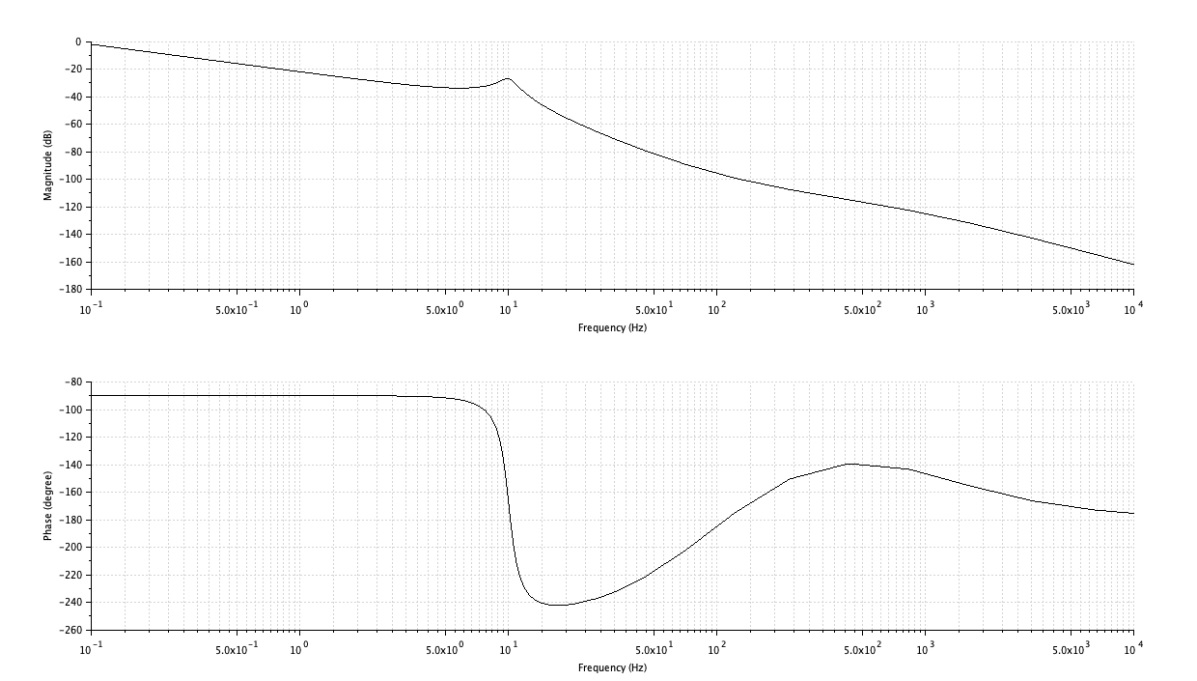
\includegraphics[width=0.6\textwidth]{Figura1.jpg}
  \caption{Respuesta en Frecuencia del Sistema en análisis.}
  \label{fig:ejemplo}
\end{figure}

Se desean diseñar diferentes sistemas de control que se adapten y mejoren el comportamiento de lazo cerrado del mismo y que cumplan con las siguientes especificaciones:

\begin{itemize}
    \item Error cero cuando la referencia es un escalón.
    \item Error menor al 10$\%$ cuando la referencia es una rampa.
    \item Margen de fase mayor o igual a 60$^\circ$, de tal forma que al aproximar el sistema en lazo cerrado a un sistema de segundo orden se obtenga un spbreimpulso no mayor al 20$\%$.
\end{itemize}

El diagrama presentado en la Figura 2 permite visualizar un acercamiento al pico máximo de resonancia del sistema y su respectiva frecuencia.\\

\begin{figure}
  \centering
    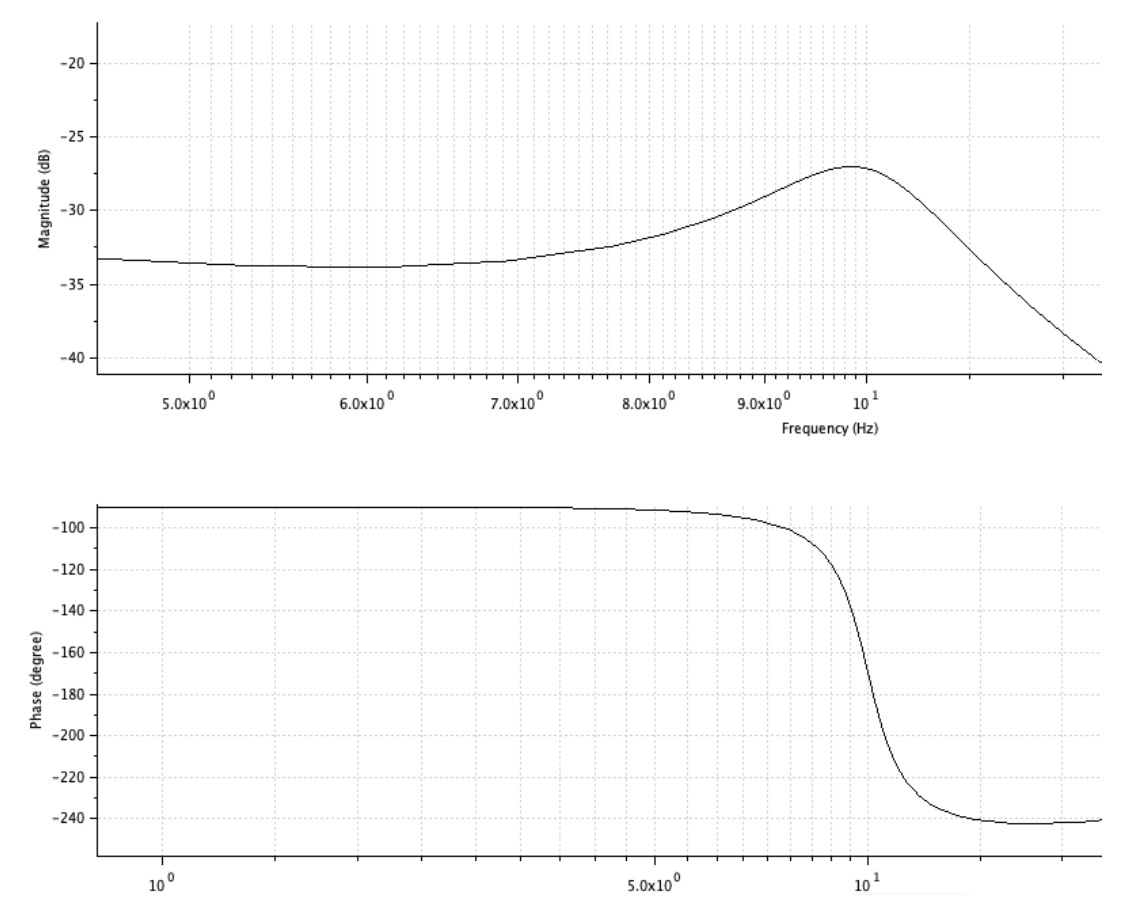
\includegraphics[width=0.6\textwidth]{Fig2.jpg}
  \caption{Zoom del pico de resonancia máxima y su frecuencia.}
  \label{fig:ejemplo}
\end{figure}


A continuación se presentan algunas relaciones de interés para el desarrollo de los diseños:

\begin{equation}
    \xi = \frac{MF}{100}
\end{equation}

\begin{equation}
    M_r = \frac{1}{2\xi\sqrt{1-\xi^2}}
\end{equation}

\begin{equation}
    \omega_r = \omega_n \sqrt{1-2\xi^2}
\end{equation}

\begin{equation}
    M_p = \exp^\frac{-\pi\xi}{\sqrt{1-\xi2}}
\end{equation}


\begin{equation}
    e_{ss}= \lim_{s \to 0} \frac{sR(s)}{1+G(s)H(s)}
\end{equation}


Donde $\xi$ es el factor de amortiguamiento, MF es el Margen de Fase, $M_r$ el pico máximo de ganancia a la frecuencia de resonancia $\omega_r$, $M_p$ el sobreimpulso y $e_{ss}$ el error de estado estacionario que depende de la entrada R(s). Se puede además estimar de forma aproximada el tiempo de levantamiento como t_r $\approx$ 1.8/$\omega_n$. Además se recuerda que el ancho de banda se determina en la frecuencia de -3dB.

\section{Cuestionamientos}
1. Asumiendo que H(s) = 1. Encuentre la función de transferencia de lazo abierto a partirde los diagramas de Bode proporcionados.\\

\textbf{Solución}

Llámese a la función de transefencia buscada G(s). Tomándo como base los puntos de interés marcados en base a la Figura 1, representados en la Figura 3, y observándose que en el punto 1 (de la Figura 3):

\begin{equation*}
    M_r \approx -27,03125 dB
\end{equation*}


Sustutiyendo el valor de $M_r$ en la ecuación (2) se tiene que:

\begin{equation*}
    \xi \approx -0.0839
\end{equation*}

\begin{figure}
  \centering
    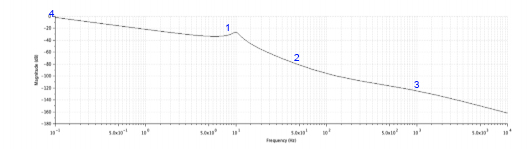
\includegraphics[width=0.8\textwidth]{diag3.jpg}
  \caption{Respuesta en Frecuencia del Sistema en análisis con los puntos de interés}
  \label{fig:ejemplo}
\end{figure}


De igual forma utilizando la ecuación (3), despejando $\omega_n$ con el valor de $\xi$ obtenido anteriormente:

\begin{equation*}
    \omega_n = 61.8059
\end{equation*}


Además obsérvece que el punto 1 es un polo doble, por lo tanto:

\begin{equation}
    G(s)= ((\frac{s}{\omega_n})^2 + 2\frac{\xi}{\omega_n}s +1) = ((\frac{s}{61.8059})^2 +2*\frac{-0.0839}{61.8059}s + 1)
\end{equation}

Analizando el punto de referencia 2, de la Figura 3; se trazan líneas tangentes en la curva para determinar la existencia de otros polos.

En el punto 3, de la Figura 3, el polo se ajustó con la gráfica de fase, donde en $10^4$ Hz es -175$\^°$ y el pico máximo que llega a 140$\^°$.

Por lo tanto la función de transferencia del sistema queda como:

\begin{equation}
    G(s) = \frac{0.45+ 0.0009217s}{0.000000004.629s^4+0.0002677s^3+0.0338937s^2 +s}
\end{equation}

Para ingresar la Función de Transferencia a \textbf{Scilab} se utilizaron varios comandos. En primer lugar, para definir a la variable \textit{s} se usó:

\begin{verbatim}
    s= poly(0, 's')
\end{verbatim}

Una vez definido \textit{s} como variable de estado, se procedió a crear la función de transferencia como:

\begin{verbatim}
    Gs= syslin('c', G(s))
\end{verbatim}

Donde G(s)= corresponde a la función de transferencia en la ecuación (7).\\

\\
\\
%------------------Inciso 2----------------%
2. Determine el error de estado estacionario del sistema.\\
\\
\textbf{Solución}\\


\textbf{NOTA: G(s) = FT} para los archivos de Scilab.
Utilizando el comando para determinar el error de estado estacionario de \textit{Scilab}, css:

\begin{verbatim}
    css = horner(s*FT*Rs, 0)
\end{verbatim}

Donde Rs es una entrada escalón unitario $Rs = \frac{1}{s}$, se obtuvo que el error de estado estacionario es:
\begin{equation}
    e_{ss} \to \infty
\end{equation}
\\

%------------------Inciso 3----------------%
3. Determine el error en estado estacionario en lazo cerrado (Scilab).\\
\\
\textbf{Solución}\\

Cerrando el lazo mediante:

\begin{verbatim}
    css = horner(s*Rs/(1+FT), 0)
\end{verbatim}

\begin{equation}
    e_{ss} = 0
\end{equation}
\\

%------------------Inciso 4----------------%
4. Utilizando el Diagrama de Nyquist, evalúe la estabilidad en lazo cerrado $L(s) = G(s)H(s)$. (Scilab).\\
\\
\textbf{Solución}\\
Para evaluar la estabilidad en lazo cerrado se ocupa saber si existe algún cero en el lado derecho del plano, para ello se obtiene el diagrama de Nyquist de la función en lazo abierto, asi, de esta forma logramos 

\begin{figure}
  \centering
    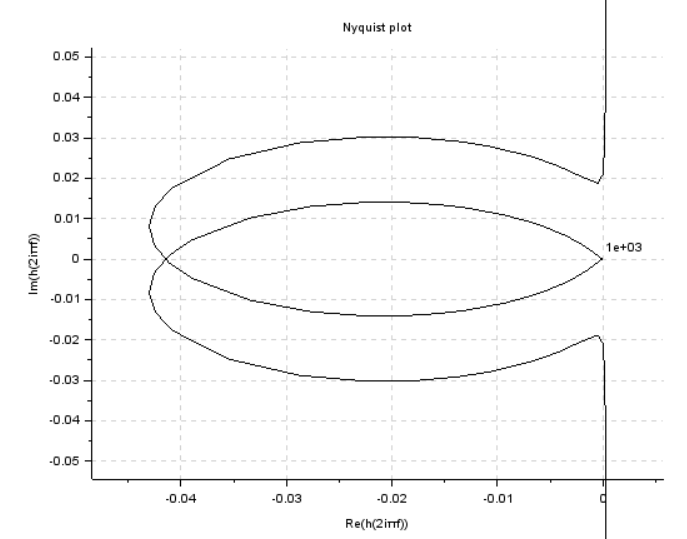
\includegraphics[width=0.8\textwidth]{4nyquist_FT.png}
  \caption{Diagrama de Nyquist para lazo abierto del sistema}
  \label{Nyq}
\end{figure}


%------------------Inciso 5----------------%
5. Diseñe un compensador tipo PD y evalúe la estabilidad del sistema para las entradas solicitadas, además corrobore si se cumplen las especificaciones de diseño a través de la carta de Nichols.\\

\textbf{Solución}\\




A partir del código siguiente se generó el diagrama de Nichols del Sistema al agregar los controladores. Obsérvese la Figura 4

\begin{verbatim}
    FT_PD = PD*FT
black(FT_PD)
nicholschart(colors=color('green')*[1,1])
/////// PI

disp("-----------")
disp(" 	PD	")
disp("-----------")


/////// PID

disp("-----------")
disp(" 	PID	")
disp("-----------")

\end{verbatim}

\begin{figure}
  \centering
    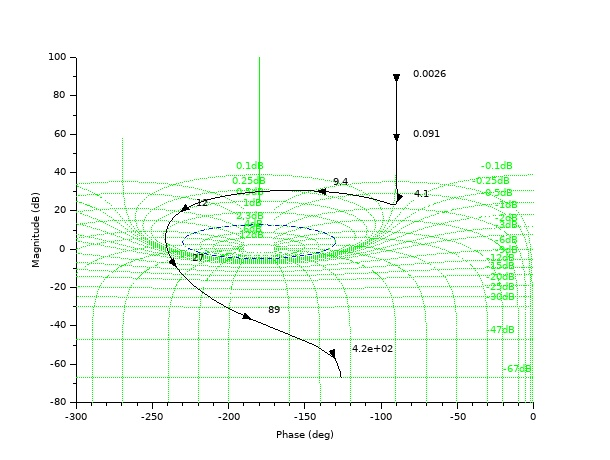
\includegraphics[width=0.8\textwidth]{nichols.jpg}
  \caption{Diagrama de Nichols del sistema compensado.}
  \label{fig:ejemplo}
\end{figure}


%------------------Inciso 6----------------%
6. Grafique la respuesta a las dos entradas solicitadas (escalón y rampa) con el compensador PD diseñado, además calcula el error de estado estacionario.\\
\textbf{Solución}\\




%------------------Inciso 7----------------%
7. Trace el diagrama de Bode de lazo cerrado con el compensador disẽnado en (5) y comparelo con la
carta de Nichols obtenida en (5) gŕaficamente. (SCilab).\\

\textbf{Solución}\\






%------------------Inciso 8----------------%
8. Repita los puntos (5) y (6) para un compensador PI, PID, de adelanto y de atraso.\\

\textbf{Solución}\\





%----------------Inciso 9----------------%
9. Realice un ańalisis comparativo en el informe de los resultados obtenidos en los puntos del (5) al (7)
entre los reguladores obtenidos.¿Cúal regulador es el mejor?\\

\textbf{Solución}\\



%------------------Inciso 10-------------%
10. En todos los cuestionamientos utilice la herramienta Scilab, y coloque en el informe los comandos (scripts) que utiliźo para desarrollar cada respuesta, y utilice las gŕaficas resultantes para detallar su ańalisis y conclusiones\\

\section{Analisis de resultados}

Para obtener la función de transferencia desde el diagrama de bode se utilizaron varios métodos gráficos de forma tal que se obtuvo un $\omega_n=9.8Hz$, un $\gamma=0.09$

\begin{equation}
    z = 0
    \label{nombre}
\end{equation}


\nocite{*}
\bibliographystyle{ieeetr}
\bibliography{main.bib}
\end{document}




